\documentclass{standalone}
\usepackage{tikz}
\usetikzlibrary{patterns, positioning}

\begin{document}
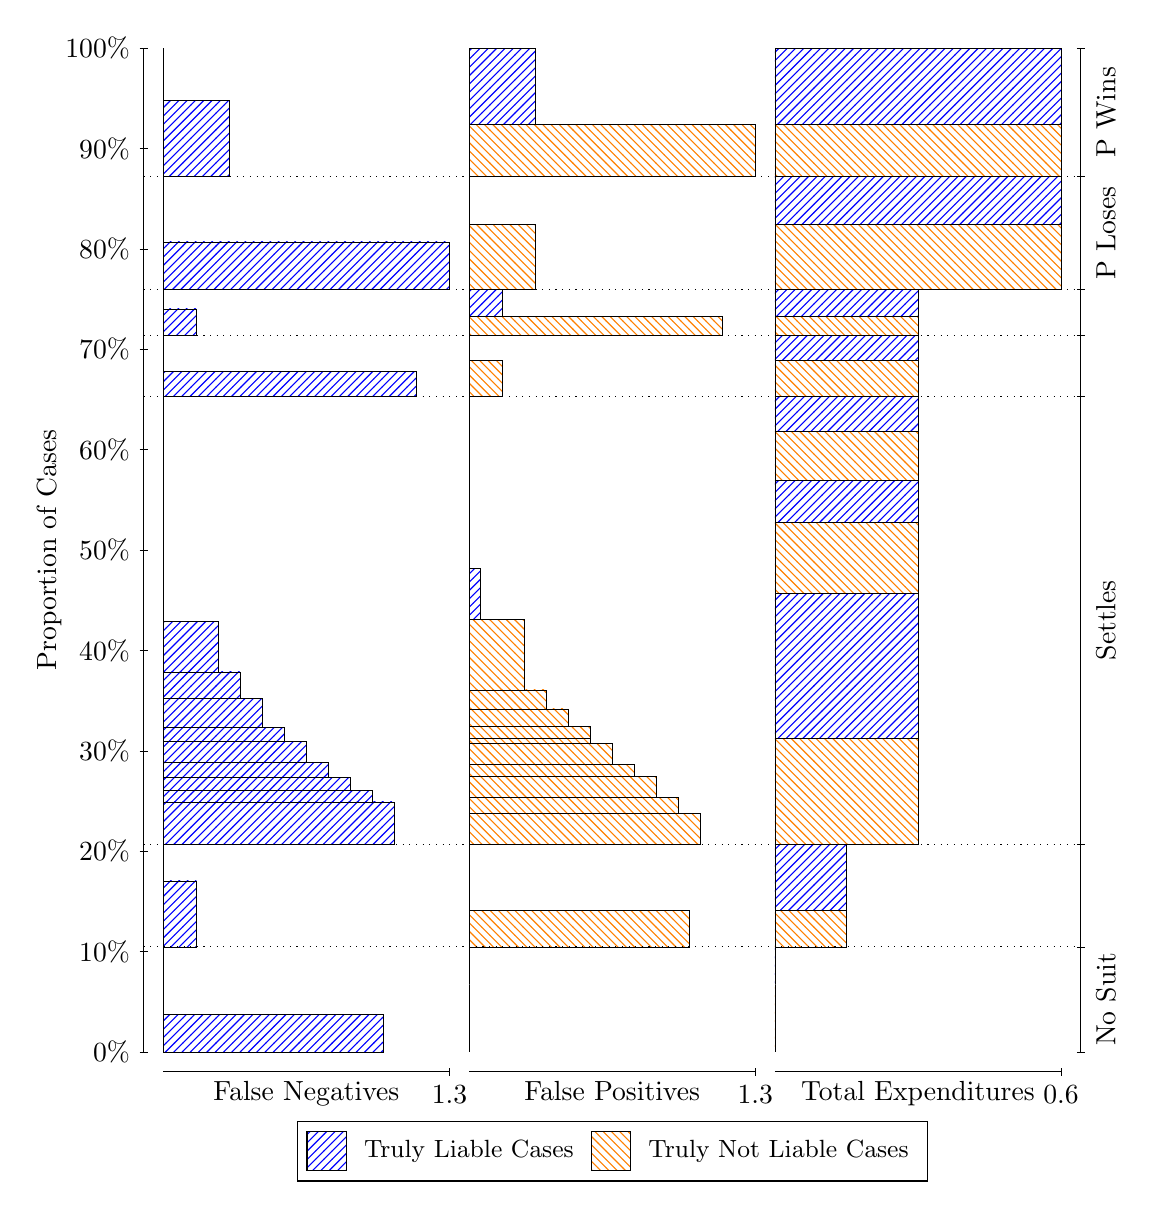
\begin{tikzpicture}
\draw[black, very thin] (1.5,1.75) -- (1.5,14.5);
\node[rotate=90, anchor=center] at (0.3, 8.125) {Proportion of Cases};
\draw[black, very thin] (1.45,1.75) -- (1.55,1.75);
\node[anchor=east] at (1.45, 1.75) {0\%};
\draw[black, very thin] (1.45,3.025) -- (1.55,3.025);
\node[anchor=east] at (1.45, 3.025) {10\%};
\draw[black, very thin] (1.45,4.3) -- (1.55,4.3);
\node[anchor=east] at (1.45, 4.3) {20\%};
\draw[black, very thin] (1.45,5.575) -- (1.55,5.575);
\node[anchor=east] at (1.45, 5.575) {30\%};
\draw[black, very thin] (1.45,6.85) -- (1.55,6.85);
\node[anchor=east] at (1.45, 6.85) {40\%};
\draw[black, very thin] (1.45,8.125) -- (1.55,8.125);
\node[anchor=east] at (1.45, 8.125) {50\%};
\draw[black, very thin] (1.45,9.4) -- (1.55,9.4);
\node[anchor=east] at (1.45, 9.4) {60\%};
\draw[black, very thin] (1.45,10.675) -- (1.55,10.675);
\node[anchor=east] at (1.45, 10.675) {70\%};
\draw[black, very thin] (1.45,11.95) -- (1.55,11.95);
\node[anchor=east] at (1.45, 11.95) {80\%};
\draw[black, very thin] (1.45,13.225) -- (1.55,13.225);
\node[anchor=east] at (1.45, 13.225) {90\%};
\draw[black, very thin] (1.45,14.5) -- (1.55,14.5);
\node[anchor=east] at (1.45, 14.5) {100\%};

\draw[black, very thin] (13.4,1.75) -- (13.4,14.5);
\draw[black, very thin] (13.35,1.75) -- (13.45,1.75);
\node[anchor=west] at (13.35, 1.75) {};
\draw[black, very thin] (13.35,3.0846) -- (13.45,3.0846);
\node[anchor=west] at (13.35, 3.0846) {};
\draw[black, very thin] (13.35,4.3852) -- (13.45,4.3852);
\node[anchor=west] at (13.35, 4.3852) {};
\draw[black, very thin] (13.35,10.08) -- (13.45,10.08);
\node[anchor=west] at (13.35, 10.08) {};
\draw[black, very thin] (13.35,10.849) -- (13.45,10.849);
\node[anchor=west] at (13.35, 10.849) {};
\draw[black, very thin] (13.35,11.433) -- (13.45,11.433);
\node[anchor=west] at (13.35, 11.433) {};
\draw[black, very thin] (13.35,12.869) -- (13.45,12.869);
\node[anchor=west] at (13.35, 12.869) {};
\draw[black, very thin] (13.35,14.5) -- (13.45,14.5);
\node[anchor=west] at (13.35, 14.5) {};

\draw[black, very thin, pattern color=blue, pattern=north east lines] (1.75,1.75) rectangle (4.5449,2.2285);
\draw[black, very thin, pattern color=orange, pattern=north west lines] (1.75,2.2285) rectangle (1.75,3.0846);
\draw[black, very thin, pattern color=blue, pattern=north east lines] (1.75,3.0846) rectangle (2.1692,3.9234);
\draw[black, very thin, pattern color=orange, pattern=north west lines] (1.75,3.9234) rectangle (1.75,4.3852);
\draw[black, very thin, pattern color=blue, pattern=north east lines] (1.75,4.3852) rectangle (4.6846,4.9263);
\draw[black, very thin, pattern color=blue, pattern=north east lines] (1.75,4.9263) rectangle (4.4051,5.0742);
\draw[black, very thin, pattern color=blue, pattern=north east lines] (1.75,5.0742) rectangle (4.1256,5.2412);
\draw[black, very thin, pattern color=blue, pattern=north east lines] (1.75,5.2412) rectangle (3.8462,5.4295);
\draw[black, very thin, pattern color=blue, pattern=north east lines] (1.75,5.4295) rectangle (3.5667,5.6962);
\draw[black, very thin, pattern color=blue, pattern=north east lines] (1.75,5.6962) rectangle (3.2872,5.8701);
\draw[black, very thin, pattern color=blue, pattern=north east lines] (1.75,5.8701) rectangle (3.0077,6.2435);
\draw[black, very thin, pattern color=blue, pattern=north east lines] (1.75,6.2435) rectangle (2.7282,6.5772);
\draw[black, very thin, pattern color=blue, pattern=north east lines] (1.75,6.5772) rectangle (2.4487,7.2174);
\draw[black, very thin, pattern color=orange, pattern=north west lines] (1.75,7.2174) rectangle (1.75,10.08);
\draw[black, very thin, pattern color=blue, pattern=north east lines] (1.75,10.08) rectangle (4.9641,10.398);
\draw[black, very thin, pattern color=orange, pattern=north west lines] (1.75,10.398) rectangle (1.75,10.849);
\draw[black, very thin, pattern color=blue, pattern=north east lines] (1.75,10.849) rectangle (2.1692,11.187);
\draw[black, very thin, pattern color=orange, pattern=north west lines] (1.75,11.187) rectangle (1.75,11.433);
\draw[black, very thin, pattern color=blue, pattern=north east lines] (1.75,11.433) rectangle (5.3833,12.037);
\draw[black, very thin, pattern color=orange, pattern=north west lines] (1.75,12.037) rectangle (1.75,12.869);
\draw[black, very thin, pattern color=blue, pattern=north east lines] (1.75,12.869) rectangle (2.5885,13.835);
\draw[black, very thin, pattern color=orange, pattern=north west lines] (1.75,13.835) rectangle (1.75,14.5);
\draw[black, very thin, pattern color=orange, pattern=north west lines] (5.6333,1.75) rectangle (5.6333,2.6062);
\draw[black, very thin, pattern color=blue, pattern=north east lines] (5.6333,2.6062) rectangle (5.6333,3.0846);
\draw[black, very thin, pattern color=orange, pattern=north west lines] (5.6333,3.0846) rectangle (8.4282,3.5464);
\draw[black, very thin, pattern color=blue, pattern=north east lines] (5.6333,3.5464) rectangle (5.6333,4.3852);
\draw[black, very thin, pattern color=orange, pattern=north west lines] (5.6333,4.3852) rectangle (8.5679,4.7764);
\draw[black, very thin, pattern color=orange, pattern=north west lines] (5.6333,4.7764) rectangle (8.2885,4.987);
\draw[black, very thin, pattern color=orange, pattern=north west lines] (5.6333,4.987) rectangle (8.009,5.2504);
\draw[black, very thin, pattern color=orange, pattern=north west lines] (5.6333,5.2504) rectangle (7.7295,5.4063);
\draw[black, very thin, pattern color=orange, pattern=north west lines] (5.6333,5.4063) rectangle (7.45,5.6727);
\draw[black, very thin, pattern color=orange, pattern=north west lines] (5.6333,5.6727) rectangle (7.1705,5.7326);
\draw[black, very thin, pattern color=orange, pattern=north west lines] (5.6333,5.7326) rectangle (7.1705,5.8818);
\draw[black, very thin, pattern color=orange, pattern=north west lines] (5.6333,5.8818) rectangle (6.891,6.1085);
\draw[black, very thin, pattern color=orange, pattern=north west lines] (5.6333,6.1085) rectangle (6.6115,6.3498);
\draw[black, very thin, pattern color=orange, pattern=north west lines] (5.6333,6.3498) rectangle (6.3321,7.2476);
\draw[black, very thin, pattern color=blue, pattern=north east lines] (5.6333,7.2476) rectangle (5.7731,7.8879);
\draw[black, very thin, pattern color=blue, pattern=north east lines] (5.6333,7.8879) rectangle (5.6333,10.08);
\draw[black, very thin, pattern color=orange, pattern=north west lines] (5.6333,10.08) rectangle (6.0526,10.532);
\draw[black, very thin, pattern color=blue, pattern=north east lines] (5.6333,10.532) rectangle (5.6333,10.849);
\draw[black, very thin, pattern color=orange, pattern=north west lines] (5.6333,10.849) rectangle (8.8474,11.096);
\draw[black, very thin, pattern color=blue, pattern=north east lines] (5.6333,11.096) rectangle (6.0526,11.433);
\draw[black, very thin, pattern color=orange, pattern=north west lines] (5.6333,11.433) rectangle (6.4718,12.265);
\draw[black, very thin, pattern color=blue, pattern=north east lines] (5.6333,12.265) rectangle (5.6333,12.869);
\draw[black, very thin, pattern color=orange, pattern=north west lines] (5.6333,12.869) rectangle (9.2667,13.534);
\draw[black, very thin, pattern color=blue, pattern=north east lines] (5.6333,13.534) rectangle (6.4718,14.5);
\draw[black, very thin, pattern color=orange, pattern=north west lines] (9.5167,1.75) rectangle (9.5167,2.6062);
\draw[black, very thin, pattern color=blue, pattern=north east lines] (9.5167,2.6062) rectangle (9.5167,3.0846);
\draw[black, very thin, pattern color=orange, pattern=north west lines] (9.5167,3.0846) rectangle (10.425,3.5464);
\draw[black, very thin, pattern color=blue, pattern=north east lines] (9.5167,3.5464) rectangle (10.425,4.3852);
\draw[black, very thin, pattern color=orange, pattern=north west lines] (9.5167,4.3852) rectangle (11.333,5.7326);
\draw[black, very thin, pattern color=blue, pattern=north east lines] (9.5167,5.7326) rectangle (11.333,7.5733);
\draw[black, very thin, pattern color=orange, pattern=north west lines] (9.5167,7.5733) rectangle (11.333,8.4711);
\draw[black, very thin, pattern color=blue, pattern=north east lines] (9.5167,8.4711) rectangle (11.333,9.0122);
\draw[black, very thin, pattern color=orange, pattern=north west lines] (9.5167,9.0122) rectangle (11.333,9.6295);
\draw[black, very thin, pattern color=blue, pattern=north east lines] (9.5167,9.6295) rectangle (11.333,10.08);
\draw[black, very thin, pattern color=orange, pattern=north west lines] (9.5167,10.08) rectangle (11.333,10.532);
\draw[black, very thin, pattern color=blue, pattern=north east lines] (9.5167,10.532) rectangle (11.333,10.849);
\draw[black, very thin, pattern color=orange, pattern=north west lines] (9.5167,10.849) rectangle (11.333,11.096);
\draw[black, very thin, pattern color=blue, pattern=north east lines] (9.5167,11.096) rectangle (11.333,11.433);
\draw[black, very thin, pattern color=orange, pattern=north west lines] (9.5167,11.433) rectangle (13.15,12.265);
\draw[black, very thin, pattern color=blue, pattern=north east lines] (9.5167,12.265) rectangle (13.15,12.869);
\draw[black, very thin, pattern color=orange, pattern=north west lines] (9.5167,12.869) rectangle (13.15,13.534);
\draw[black, very thin, pattern color=blue, pattern=north east lines] (9.5167,13.534) rectangle (13.15,14.5);
\draw[black, dotted] (1.5,3.0846) -- (13.4,3.0846);
\draw[black, dotted] (1.5,4.3852) -- (13.4,4.3852);
\draw[black, dotted] (1.5,10.08) -- (13.4,10.08);
\draw[black, dotted] (1.5,10.849) -- (13.4,10.849);
\draw[black, dotted] (1.5,11.433) -- (13.4,11.433);
\draw[black, dotted] (1.5,12.869) -- (13.4,12.869);
\draw[black, very thin] (1.75,1.5) -- (5.3833,1.5);
\node[anchor=north] at (3.5667, 1.5) {False Negatives};
\draw[black, very thin] (5.3833,1.45) -- (5.3833,1.55);
\node[anchor=north] at (5.3833, 1.45) {1.3};

\draw[black, very thin] (5.6333,1.5) -- (9.2667,1.5);
\node[anchor=north] at (7.45, 1.5) {False Positives};
\draw[black, very thin] (9.2667,1.45) -- (9.2667,1.55);
\node[anchor=north] at (9.2667, 1.45) {1.3};

\draw[black, very thin] (9.5167,1.5) -- (13.15,1.5);
\node[anchor=north] at (11.333, 1.5) {Total Expenditures};
\draw[black, very thin] (13.15,1.45) -- (13.15,1.55);
\node[anchor=north] at (13.15, 1.45) {0.6};

\node[black, centered, rotate=90] at (13.72, 2.4173) {No Suit};

\node[black, centered, rotate=90] at (13.72, 7.2325) {Settles};


\node[black, centered, rotate=90] at (13.72, 12.151) {P Loses};
\node[black, centered, rotate=90] at (13.72, 13.684) {P Wins};

\draw (7.449999999999999,1.5) node[draw=none] (baseCoordinate) {};
\begin{scope}[align=center]
        \matrix[scale=0.5, draw=black, below=0.5cm of baseCoordinate, nodes={draw}, column sep=0.1cm]{
            \node[rectangle, draw, minimum width=0.5cm, minimum height=0.5cm, pattern=north east lines, pattern color=blue] {}; &
            \node[draw=none, font=\small] (B) {Truly Liable Cases}; &
            \node[rectangle, draw, minimum width=0.5cm, minimum height=0.5cm, pattern=north west lines, pattern color=orange] {}; &
            \node[draw=none, font=\small] (B) {Truly Not Liable Cases}; \\
            };
\end{scope}

\end{tikzpicture}
\end{document}